\chapter{変分量子アルゴリズム}\label{chap:vqa}
この章では、NISQ 上でも実行可能なアルゴリズムとして現在盛んに研究されいてる変分量子アルゴリズムについて説明する。\ref{sec:vqc}~節では、変分量子アルゴリズムをコスト関数・変分量子回路・最適化の3つ部分に分けて説明する。\ref{sec:qml}~節では、量子機械学習について説明する。\ref{sec:bp}~節では、バレンプラトーについて説明する。

\section{概要}\label{sec:vqc}
現在実現されている量子コンピューターは、中規模(数百量子ビット)であり、ノイズが大きいため、Noisy Intermediate Scale Quantum computers (\ruby{NISQ}{ニスク})と呼ばれている\cite{preskill2018quantum}。このため、使用できる量子ビットと量子ゲートの数に制約がある。そのような制約のもと、古典計算よりも効率的に計算を行うことを期待されているのが、変分量子アルゴリズムである。
変分量子アルゴリズムは、古典コンピューターと組み合わせて最適化問題を解くアルゴリズムである。最適化問題とは、ある関数の値を最小化するようなパラメーターの値を求める問題である。
変分量子アルゴリズムでは、パラメーターに依存した量子状態によってオブザーバブルの期待値を計算し、それを用いて定義されたコスト関数 $C(\bs{\th})$ を最適化することによって問題を解く。
パラメーターの更新を古典コンピューターに任せることで、量子回路を浅く保つことができる。図\ref{fig:vqa-flow}のように、量子状態の生成からパラメーターの更新までのサイクルを繰り返すことで、最終的に最適なパラメーター$\bs{\th}_* = \argmin_{\bs{\th}} C(\bs{\th})$ を得る。試行関数を生成するパラメーター付き量子回路のことを、変分量子回路、アンザッツ(Ansatz)、あるいは、量子ニューラルネットワーク(Quanum Neural Network, QNN)と呼ぶ。
\begin{figure}[H]
    \centering
    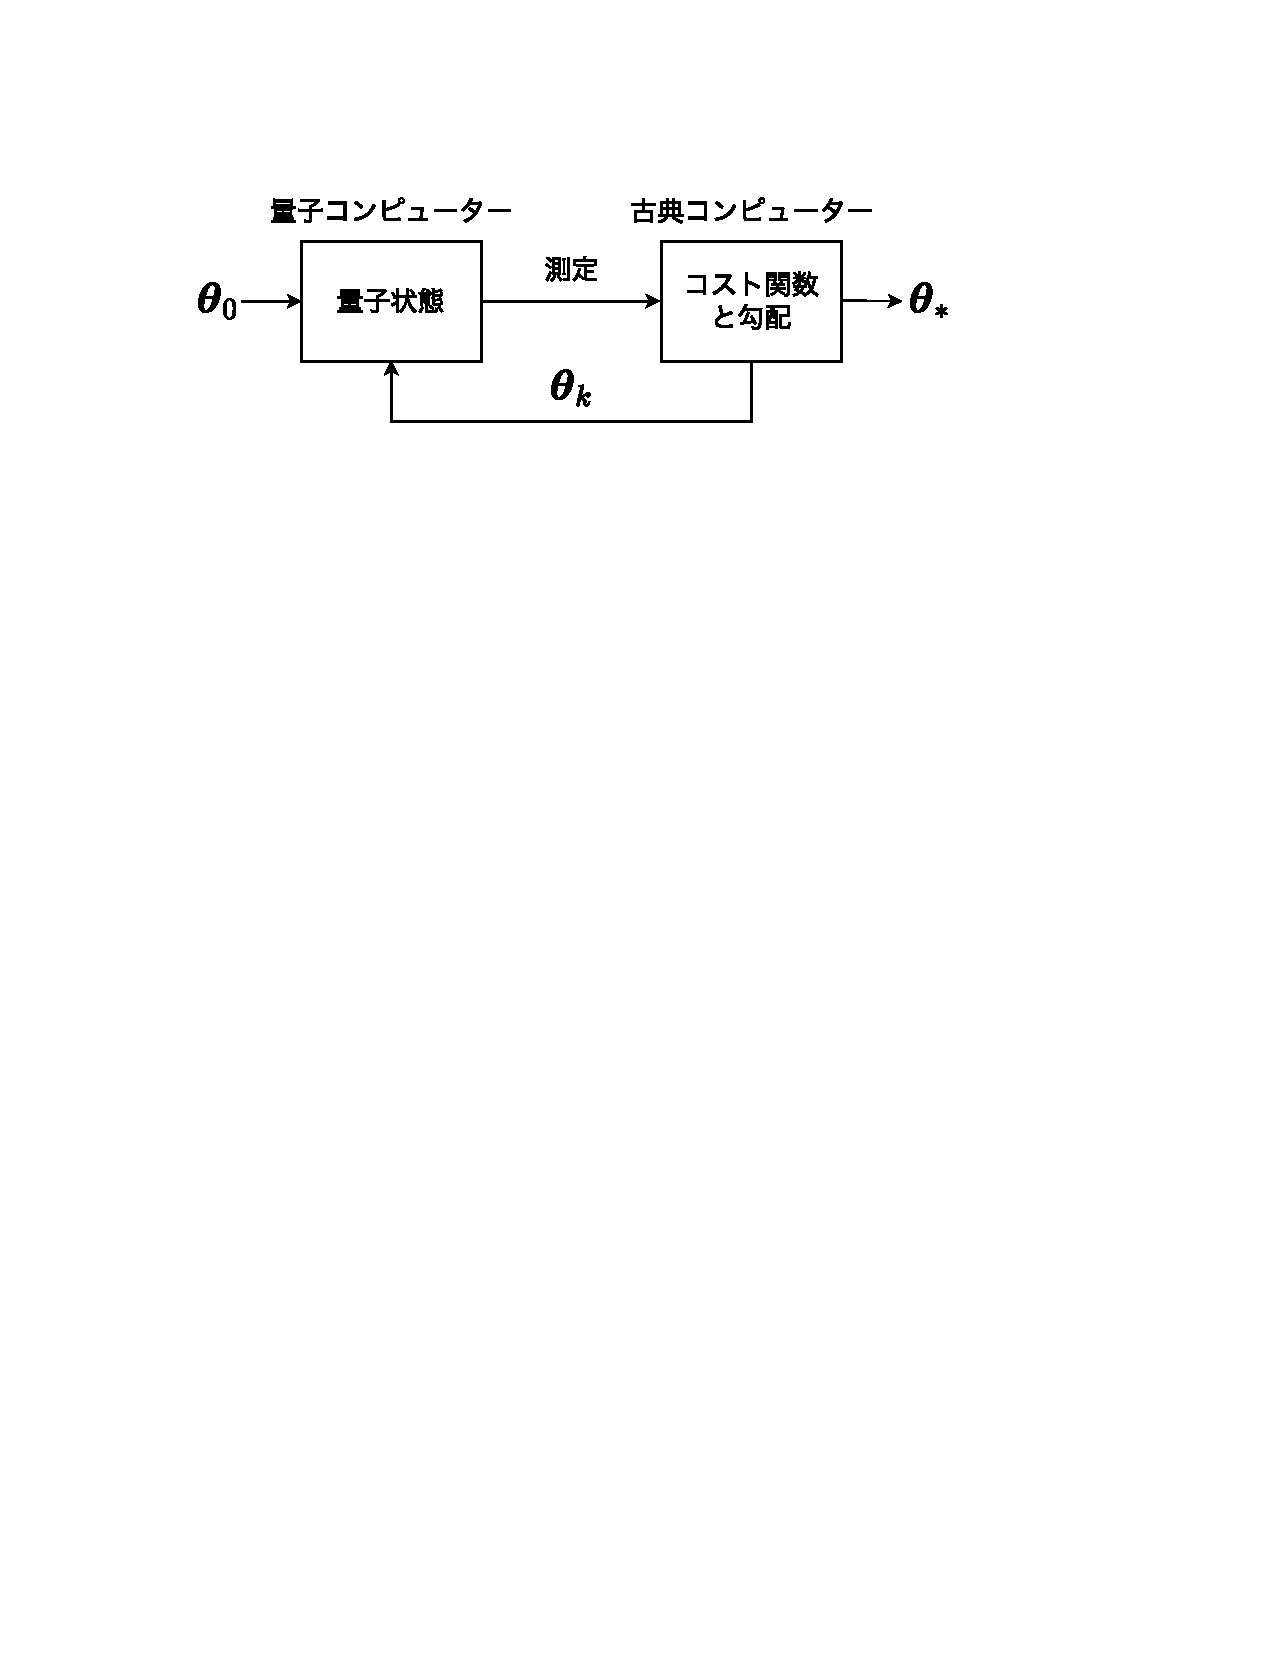
\includegraphics[width=12cm]{vqa-flow.pdf}
    \caption{変分量子アルゴリズムの概要}
    \label{fig:vqa-flow}
\end{figure}

ある問題を解くための変分量子アルゴリズムを構成するには、以下の3つの要素が必要である。
\begin{enumerate}
    \item 解きたい問題をコスト関数の最適化問題として定式化すること
    \item コスト関数を最適化するための変分量子回路を構成すること
    \item パラメーターを最適化するための最適化手法を選択すること
\end{enumerate}
これらについて、順に説明する。

\subsection{コスト関数}\label{sec:cost}
変分量子アルゴリズムにおけるコスト関数は、初期状態の集合 $\{\rho_i\}$、変分量子回路 $V(\bs{\th})$、オブザーバブルの集合 $\{O_k\}$ を用いて定義される。変分量子回路を作用させた状態 $V(\bs{\th}) \rho_i V\dg(\bs{\th})$ によるオブザーバブル $O_k$ の期待値は、
\begin{align}
    \Tr[V(\bs{\th}) \rho_i V\dg(\bs{\th}) O_k]
\end{align}
である。
コスト関数は、この期待値を用いて定義される。
ほとんどのコスト関数は、$f$ を任意の関数として次のような形で与えられる。
\begin{align}\label{eq:cost-general}
    C(\bs{\th}) = f\qty(\qty{\Tr[V(\bs{\th}) \rho_i V\dg(\bs{\th}) O_k]}_{i,k})
\end{align}

コスト関数は、その最小点が求める解に対応するように設計する。
例えば、変分量子固有値ソルバー (Variational Quantum Eigensolover, VQE) では、ハミルトニアンが $H$ で与えられる系の最小エネルギーを求めるために、$\rho_i = \dyad{\psi_0}$, $O_k = H$ とする。このとき、コスト関数は以下のように定義される。
\begin{align}\label{eq:cost-vqe}
    C(\bs{\th}) = \bra{\psi_0}V\dg(\bs{\th}) H V(\bs{\th})\ket{\psi_0}
\end{align}

また、変分量子回路を用いた機械学習(量子機械学習)では、データセット $\{(\bs{x}_i, y_i)\}_{i=1}^N$ が与えられたとき、入力状態を $\rho_i = U({\bs{x}_i})\dyad{0}U\dg({\bs{x}_i})$, オブザーバブルを $O_k = O$ として、各データに依存するオブザーバブルの期待値 $\Tr[V(\bs{\th}) \rho_i V\dg(\bs{\th}) O]$ が対応するラベル $y_i$ になるように、以下のようなコスト関数を定義することができる。
\begin{align}\label{eq:cost-qml}
    C(\bs{\th}) = \frac1N\sum_{i=1}^N \qty(\Tr[V(\bs{\th}) \rho_i V\dg(\bs{\th}) O] - y_i)^2
\end{align}


\subsection{変分量子回路}
一般に、変分量子回路 $V(\bs{\th})$ は、回転ゲートなどのパラメーター付き量子ゲートと CNOT ゲートなどのパラメーターなし量子ゲートの積で表すことができる。$U_j(\bs{\th}_j)$ を任意の数のパラメーター付き量子ゲートからなるユニタリ、$W_j$ を任意の数のパラメーターなし量子ゲートからなるユニタリであるとすると、$V(\bs{\th})$ は次のように表わすことができる。
\begin{align}
    V(\bs{\th})
    = \prod_{j=1}^{L} U_j(\bs{\th}_j) W_j
    = U_L(\bs{\th}_L)W_L\cdots U_1(\bs{\th}_1)W_1
\end{align}
変分量子回路においては、類似した構造を複数回繰り返すことがあり、その構造単位の繰り返しの数を層数と呼び、この数が多いほど深い回路であるという。図~\ref{fig:vqc}は $L$ 層の変分量子回路を表している。

\newcommand{\wj}[1]{\gate[wires=3]{{\LARGE W_{#1}}}}
\newcommand{\uj}[1]{\gate[wires=3]{{\LARGE U_{#1}(\th_{#1})}}}
\begin{figure}[H]
    \centering
    \begin{quantikz}
        \lstick{$\ket{0}$}    & \wj{1}& \uj{1} & \wj{2}& \uj{2}& \ \cdots\ & \wj{L}& \uj{L}& \meter{}\\
        \lstick{$\vdots\;\;$} & \wn   & \wn    & \wn   & \wn   & \wn\cdots & \wn   & \wn   & \wn\rstick{$\vdots$}\\
        \lstick{$\ket{0}$}    &       &        &       &       & \ \cdots\ &       &       & \meter{}
    \end{quantikz}
    \caption{$L$ 層の変分量子回路}
    \label{fig:vqc}
\end{figure}

アンザッツの構造は、問題の性質に応じて様々なものが考えられる。問題の対称性や制約を構造に取り入れたアンザッツを Problem-inspired アンザッツと呼ぶ。例えば、Quantum Alternating Operator Ansatz (QAOA) は組合せ最適化問題に対して提案された Problem-inspired アンザッツである。
一方、問題の性質に依存しないアンザッツを Problem-agnostic アンザッツと呼ぶ。

Hardware Efficient Ansatz は量子コンピューターの実機の構造を考慮し、実装が効率的にできるよう設計された Problem-agnostic アンザッツである。例えば、量子ビット $q_1,\,q_2,\,q_3,\,q_4$ が隣り合うインデックスのみ実機上でつながっているときに、図~\ref{fig:hea}のような回路の構造を持つアンザッツである。
これにより、実機上で隣り合わない量子ビットを結ぶための量子ゲートを実装する必要がなくなり、使用するSWAPゲートの数が減る。SWAP ゲートは CNOT ゲート3つから成るが、CNOT ゲートは量子ゲートの中でも特にノイズが多い。そのため、SWAP ゲートを減らすことはノイズの対策として有用である。

\begin{figure}[H]
    \centering
    \begin{quantikz}
        \lstick{$q_1$} & \gate{U(\th_1)} & \ctrl{1}&  \qw    & \qw     & \gate{U(\th_5)} & \ctrl{1}&  \qw    & \qw     & \gate{U(\th_9)}    & \ctrl{1} &  \qw    & \qw     & \meter{} \\
        \lstick{$q_2$} & \gate{U(\th_2)} & \targ{} & \ctrl{1}& \qw     & \gate{U(\th_6)} & \targ{} & \ctrl{1}& \qw     & \gate{U(\th_{10})} & \targ{} & \ctrl{1}& \qw     & \meter{} \\
        \lstick{$q_3$} & \gate{U(\th_3)} & \qw     & \targ{} & \ctrl{1}& \gate{U(\th_7)} & \qw     & \targ{} & \ctrl{1}& \gate{U(\th_{11})} & \qw     & \targ{} & \ctrl{1}& \meter{} \\
        \lstick{$q_4$} & \gate{U(\th_4)} & \qw     &   \qw   & \targ{} & \gate{U(\th_8)} & \qw     &   \qw   & \targ{} & \gate{U(\th_{12})} & \qw     &   \qw   & \targ{} & \meter{}
    \end{quantikz}
    \caption{Hardware Efficient Ansatz}
    \label{fig:hea}
\end{figure}


\subsection{最適化}\label{sec:optimization}
最適化とは、コスト関数を最小化するパラメーターを求めることであり、変分量子アルゴリズムでは古典コンピューターによって行われる。
最適化のアルゴリズムのことを、オプティマイザーと呼ぶ。
変分量子アルゴリズムにおいては、従来の古典計算で用いられるオプティマイザーをそのまま用いることができるが、量子計算に合わせて改良されたオプティマイザーも提案されている。オプティマイザーには、ノイズや測定誤差に強いものを選択する必要がある。

オプティマイザーには、コスト関数の勾配を用いるものと、用いないものに大別される。
勾配を用いるオプティマイザーには、勾配降下法、ニュートン法、量子自然勾配法\cite{stokes2020quantum}、確率的勾配降下法\cite{sweke2020stochastic}、Adam\cite{kingma2017adam}、などの方法がある。
勾配自体は、有限差分法やパラメーターシフトルール\cite{mitarai2018quantum,schuld2019evaluating}によって求めることができる。
例えば、勾配降下法では、パラメーター $\th_j$ を以下のように更新する。
\begin{align}
    \th_j \leftarrow \th_j - \alpha \pdv{C(\bs{\th})}{\th_j}
\end{align}
ここで、$\alpha$ は1回の更新でのパラメーターの変化量を決める、学習率と呼ばれるハイパーパラメーターである。通常、学習率は小さい正の値に設定されるが、適切な値は扱う問題によって異なる。

勾配を用いない方法では、コスト関数の値のみを用いてパラメーターを更新する。例えば、Nelder-Mead\cite{nelder1965simplex}、Powell\cite{powell1964efficient}、COBYLA (Constrained Optimization By Linear Approximation optimizer)\cite{powell1994direct}、SPSA (Simultaneous Perturbation Stochastic Approximation)\cite{spall1992multivariate}、逐次最小化問題最適化法\cite{platt1998sequential,nakanishi2020sequential,parrish2019jacobi,ostaszewski2021structure}などが挙げられる。

\subsubsection*{パラメーターシフトルール}\label{sec:parameter-shift-rule}
変分量子アルゴリズムにおいては、すべてのパラメーターが独立であれば、パラメーターシフトルールと呼ばれる手法によって、厳密に勾配を求めることができる\cite{mitarai2018quantum,schuld2019evaluating}(測定誤差は除く)。パラメーターシフトルールは、パラメーター付き量子ゲート $V(\bs{\th})$ によるオブザーバブルの期待値のパラメーター $\th_j$ に関する勾配を、パラメーター $\th_j$ を一定値ずらして得た期待値の差として求める方法である。

\begin{screen}
    \begin{theorem}
        (パラメーターシフトルール~\cite{mitarai2018quantum,schuld2019evaluating})
        % $U(\bs{\th}) := \prod_{i=1}^L U_i(\th_i)W_i = U_L(\th_L)W_L\cdots U_1(\th_1)W_1$
        量子回路 $V(\bs{\th})$ はパラメーター付き量子ゲート $U_j(\th_j) := \exp(-i\th_j P_j/2)$ とパラメーターなし量子ゲート $W_j$ によって $V(\bs{\th}) := U_L(\th_L)W_L\cdots U_1(\th_1)W_1$ と定義される。ここでは、すべてのパラメーターは独立であるとする。このとき、あるオブザーバブル $O$ の期待値 $\expval{O(\bs{\th})} = \Tr[V(\bs{\th})\dyad{0}\otn{n}V\dg(\bs{\th}) O]$ の $\th_j$ に関する勾配は
        \begin{align}
            \pdv{\expval{O(\bs{\th})}}{\th_j}
            = \frac{1}{2}\qty[\expval{O\qty({\bs{\th}}+\frac{\pi}{2}\bs{e}_j)}
            - \expval{O\qty({\bs{\th}}-\frac{\pi}{2}\bs{e}_j)}]
        \end{align}
        で与えられる。ここで $\bs{e}_j$ は $j$ 番目の方向の単位ベクトルである。
    \end{theorem}
\end{screen}

\begin{comment}
\begin{proof}
    パラメーター付き量子ゲートに対して、$U_{k:i} := U_k(\th_k)W_k \cdots U_i(\th_i)W_i$ という記法を用いる。
    $\pd_{\th_j}U_j(\th_j) = -\frac{i}{2}P_jU_j(\th_j)$ であることから、$B(\bs{\th})$ の $\th_j$ に関する勾配は、
    \begin{align}
        \pdv{\expval{B(\bs{\th})}}{\th_j}
        &= \pdv{\th_j} \Tr[BU_{L:1}\rho_{in} U_{L:1}\dg]\\
        &= \Tr[B \pdv{U_{L:1}}{\th_j} \rho_{in} U_{L:1}\dg] + \Tr[B U_{L:1} \rho_{in} \pdv{U_{L:1}\dg}{\th_j}]\\
        &= \Tr[B \qty(-\frac{i}{2}U_{L:j-1}P_jU_{j:1}) \rho_{in} U_{L:1}\dg] + \Tr[B U_{L:1} \rho_{in} \qty(\frac{i}{2}U_{j:1}\dg P_jU_{L:j-1}\dg)]\\
        &= -\frac{i}{2}\Tr[BU_{L:j-1}[P_j,U_{j:1}\rho_{in} U_{j:1}\dg]U_{L:j-1}\dg]
    \end{align}
    ここで、$U_j(\pm\pi/2) = (1/\sqrt{2})(\bbid\mp iP_j)$ であることから、
    \begin{align}
        [P_j,\rho^\prime] = i\qty[U_j\qty(\frac{\pi}{2})\rho^\prime\, U_j\qty(\frac{\pi}{2}) - U_j\qty(-\frac{\pi}{2})\rho^\prime\, U_j\qty(-\frac{\pi}{2})]
    \end{align}
    が成り立つ。
    よって、
    \begin{align}
    & U_{L:j-1}[P_j,U_{j:1}\rho_{in} U_{j:1}\dg]U_{L:j-1}\dg\\
    &= iU_{L:j-1}\qty[U_j\qty(\frac{\pi}{2})U_{j:1}\rho_{in} U_{j:1}\dg U_j\qty(\frac{\pi}{2}) - U_j\qty(-\frac{\pi}{2})U_{j:1}\rho_{in} U_{j:1}\dg U_j\qty(-\frac{\pi}{2})]U_{L:j-1}\dg\\
    &= i\Big[U_{L:j}U_j\qty(\th_j + \frac{\pi}{2})U_{j-1:1}\rho_{in} U_{j-1:1}\dg U_j\qty(\th_j + \frac{\pi}{2})U_{L:j}\dg\\
    &\quad - U_{L:j}U_j\qty(\th_j - \frac{\pi}{2})U_{j-1:1}\rho_{in} U_{j-1:1}\dg U_j\qty(\th_j - \frac{\pi}{2})U_{L:j}\dg\Big]
    \end{align}
    以上より、
    \begin{align}
        \pdv{\expval{B(\bs{\th})}}{\th_j}
        &= \frac{1}{2}\qty[ BU\qty(\bs{\th} + \frac{\pi}{2}\bs{e}_j)\rho U\dg\qty(\bs{\th} + \frac{\pi}{2}\bs{e}_j)
        - BU\qty(\bs{\th} - \frac{\pi}{2}\bs{e}_j)\rho U\dg\qty(\bs{\th} - \frac{\pi}{2}\bs{e}_j)]\\
        &= \frac{1}{2}\qty[\expval{B\qty(\bs{\th} + \frac{\pi}{2}\bs{e}_j)}
        - \expval{B\qty(\bs{\th} - \frac{\pi}{2}\bs{e}_j)}]
    \end{align}
\end{proof}
\end{comment}

より高次の勾配も同様に計算することができる。例えば、$V(\bs{\th})$ の $\th_j$ と $\th_k$ に関する勾配は、
\begin{align}
    \pdv{\expval{O(\bs{\th})}}{\th_j}{\th_k}
    = \frac12\qty[\eval{\pdv{\expval{O(\bs{\th})}}{\th_j}}_{\th_k = \th_k + \frac{\pi}{2}}
    - \eval{\pdv{\expval{O(\bs{\th})}}{\th_j}}_{\th_k = \th_k - \frac{\pi}{2}}]
\end{align}
で与えられる。

一般的なコスト関数 \eqref{eq:cost-general} の勾配については、連鎖律を用いると、
\begin{align}
    \pdv{C(\bs{\th})}{\th_j}
    = \pdv{\th_j}f\qty(\qty{\Tr[V(\bs{\th}) \rho_i V\dg(\bs{\th}) O_k]}_{i,k})
    = \sum_{i,k}\pdv{f}{\ell_{i,\bs{\th},k}}\pdv{\ell_{i,\bs{\th},k}}{\th_j}
\end{align}
となるので、$\ell_{i,\bs{\th},k}$ にパラメーターシフトルールを用いて勾配を計算することができる。
ここで、$\ell_{i,\bs{\th},k} := \Tr[V(\bs{\th}) \rho_i V\dg(\bs{\th}) O_k]$ とした。



\section{量子機械学習}\label{sec:qml}
近年、機械学習\footnote{機械学習の概要については付録の\ref{sec:machine-learning}~節に置いた。}はさまざまな分野で著しい成果を上げているが、その一方で、高い計算コストが問題となっている。そこで、機械学習の計算を量子コンピューター上で行い、計算を効率化できないか研究されている。そのような研究分野を量子機械学習(Quantum Machine Learning, QML)と呼ぶ。
量子機械学習におけるアルゴリズムの研究アプローチは次の3つがあげられる\cite{guan2021quantum}。
\begin{enumerate}
    \item 古典的な学習方法から量子的なものへの再構築
    \item 古典的な学習方法に勝る新たな量子機械学習の方法の探索
    \item 近い将来に向けた、NISQに特化した学習方法の探索
\end{enumerate}

2009年、Harrow, Hassidim, Lloyd は線形方程式を解く量子アルゴリズム(HHLアルゴリズム)を提案した~\cite{harrow2009quantum}。このアルゴリズムは、古典的なアルゴリズムよりも効率的に線形方程式を解くことが期待される量子アルゴリズムである。量子機械学習の初期の研究は、機械学習における線形代数の問題を HHL アルゴリズムによって量子コンピューター上で解くことに焦点を当てていた(1のアプローチ)。しかし、HHLアルゴリズムは量子位相推定を用いており、量子ビットと量子ゲートが数多く必要であるため、NISQ で実現できるアルゴリズムではなかった。
変分量子アルゴリズムが登場したことにより、その文脈で量子機械学習の研究が盛んになった(3のアプローチ)。
この節では、変分量子アルゴリズムとして研究されている3つの教師あり量子機械学習モデルについて説明する。量子回路学習(Quantum Circuit Learning)\cite{mitarai2018quantum,farhi2018classification}、Data reuploading\cite{perez-salinas2020data,lloyd2020quantum,schuld2021effect}、量子カーネル法(Quantum Kernel Methods)\cite{havlicek2019supervised,schuld2019quantum,schuld2021supervised}である。いずれのモデルも、図\ref{fig:vqa-flow}にある流れに従って学習を行うが、量子回路で行う計算が異なる。

\subsection{量子回路学習}\label{sec:quantum-circuit-learning}
\begin{figure}[H]
    \centering
    \begin{quantikz}
        \lstick{$\ket{0}$}     & \gate[wires=3][3cm]{{\LARGE U(\bs{x}_i)}} & \gate[wires=3][3cm]{{\LARGE V(\bs{\th})}} & \meter{}\\
        \lstick{$\vdots\;\;$}  & \wn &\wn & \wn\rstick{$\vdots$}\\
        \lstick{$\ket{0}$}     &     & \qw & \meter{}
    \end{quantikz}
    \caption{量子回路学習における量子回路の構造}
    \label{fig:qcl-circuit}
\end{figure}
% \begin{figure}[H]
%     \centering
%     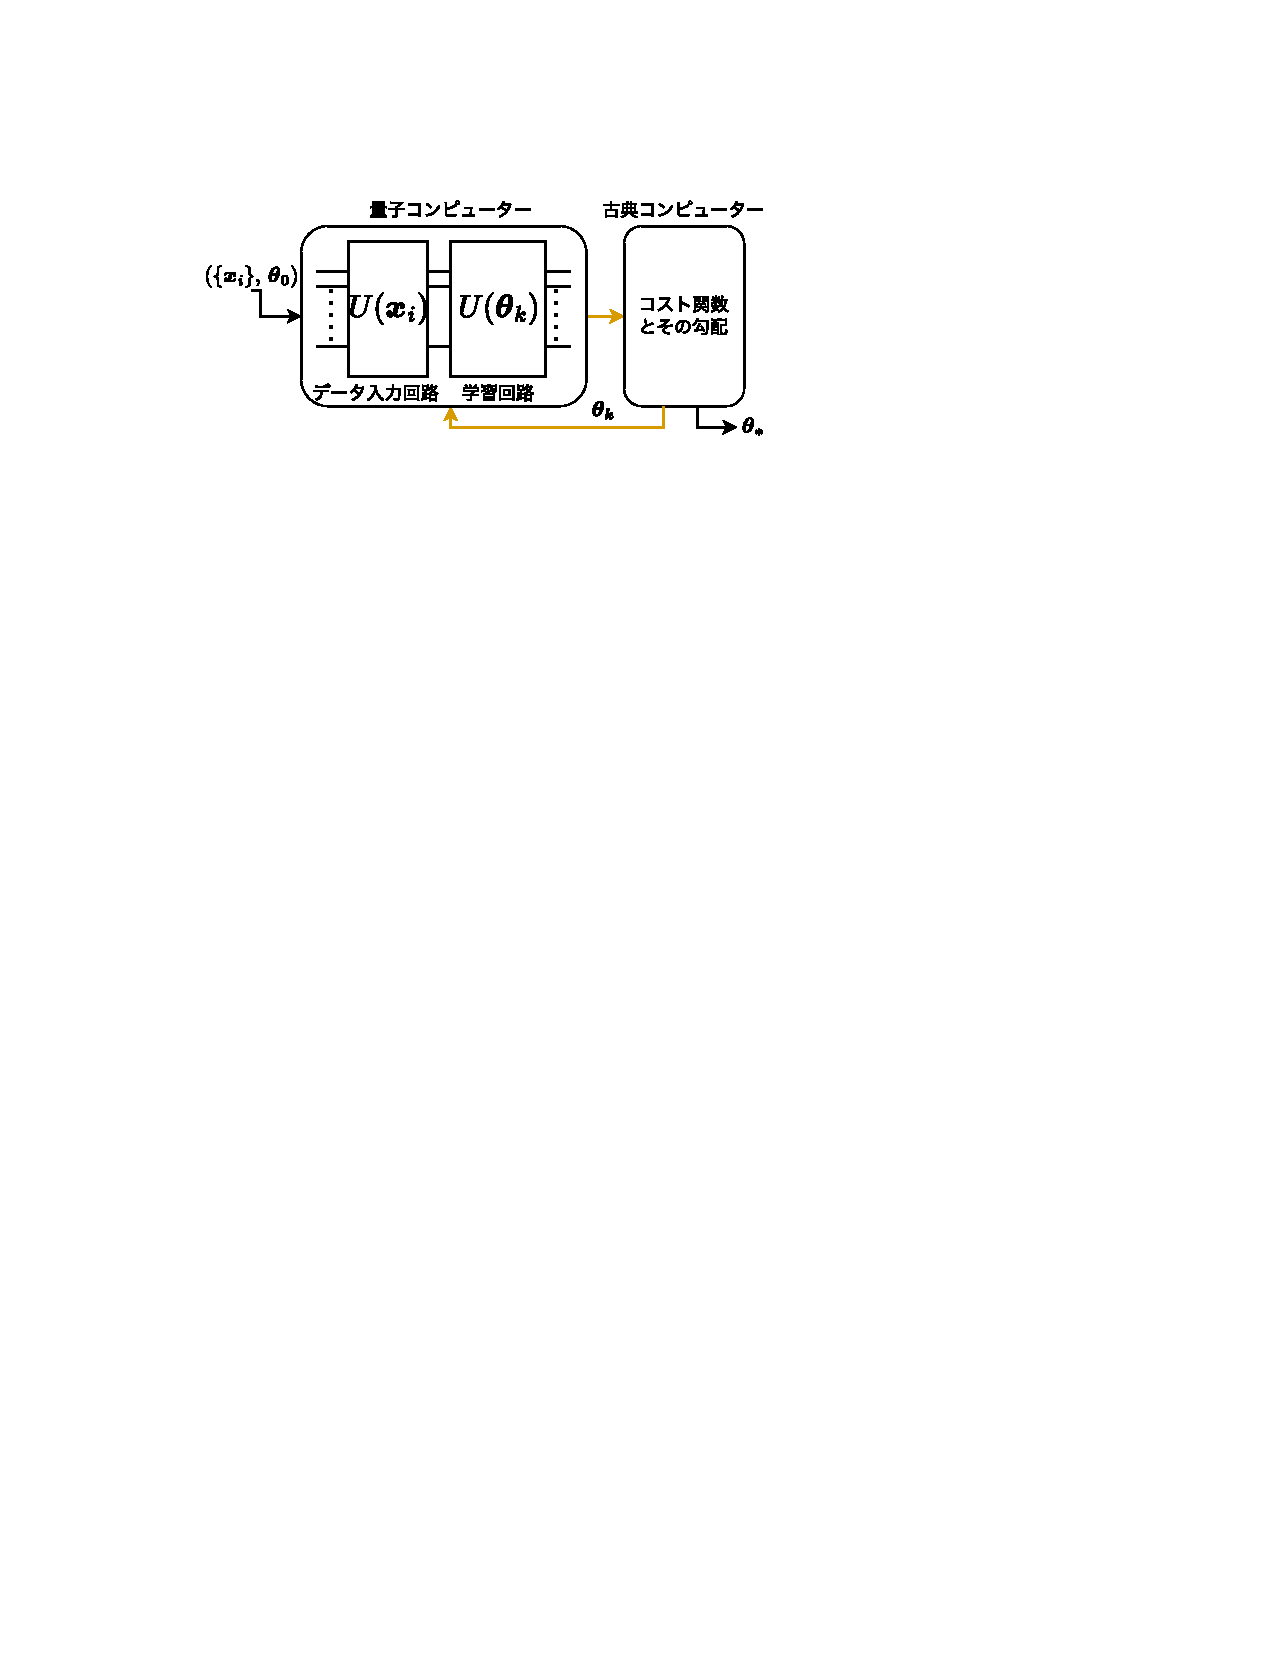
\includegraphics[width=12cm]{qml-alg.png}
%     \caption{量子回路学習の概要}
%     \label{fig:qml-alg}
% \end{figure}

図\ref{fig:qcl-circuit}は量子回路学習における量子回路の構造を表している。まず、初期状態 $\ket{0}\otn{n}$ にデータを入力するためのユニタリ $U(\bs{x}_i)$ を作用させ、続いて、学習パラメーターを入力するためのユニタリ $V(\bs{\th})$ を作用させる。前者を入力回路、後者を学習回路と呼ぶことにする。これにより、状態 $V(\bs{\th})U(\bs{x}_i)\ket{0}\otn{n}$ が生成される。
そして、この状態によって測定したオブザーバブルの期待値 $\{\Tr[V(\bs{\th})U(\bs{x}_i)\dyad{0}\otn{n}U\dg(\bs{x}_i)V\dg(\bs{\th}) O_k]\}_k$ を用いて、\ref{eq:cost-qml}のようなコスト関数が定義される。
古典コンピューター上では、コスト関数とその勾配を計算し、学習パラメーターを更新する。
このプロセスを繰り返すことで、最適なパラメーター $\bs{\th}_\ast$ を得る。
後の第\ref{chap:upper-bound},\ref{chap:lower-bound}章において扱う量子機械学習のモデルも、この量子回路学習に基づいて解析を行う。



\subsection{Data reuploading}\label{sec:data-reuploading}
\newcommand{\Ux}[1]{\gate[wires=3][1cm]{{\Large U_{#1}(\bs{x}_i,\bs{\th}_{#1})}}}
\begin{figure}[H]
    \centering
    \begin{quantikz}
        \lstick{$\ket{0}$}    &\Ux{1}&\Ux{2}&\ \ldots\    &\Ux{L}& \meter{}\\
        \lstick{$\vdots\;\;$} &\wn   &\wn   &\wn\ \ldots\ &\wn   & \wn\rstick{$\vdots$}\\
        \lstick{$\ket{0}$}    &\qw   &\qw   &\ \ldots\    &\qw   & \meter{}
    \end{quantikz}
    \caption{Data reuploading における量子回路の構造}
    \label{fig:data-reuploading}
\end{figure}

量子回路学習とは異なり、いくつかの研究においては、データの入力と学習パラメーターの入力を交互に繰り返す量子回路\cite{schuld2021effect,lloyd2020quantum}や、一つのゲートにデータと学習パラメーターの線形和を入力する量子回路\cite{perez-salinas2020data}が用いられている。このような量子回路の構造は、Data reuploading と呼ばれている(図~\ref{fig:data-reuploading})。コスト関数の定式化は、量子回路学習と同様である。




\subsection{量子カーネル法}\label{sec:quantum-kernel}
\begin{figure}[H]
    \centering
    \begin{quantikz}
        \lstick{$\ket{0}$} & \gate[wires=3][3cm]{{\LARGE U(\bs{x}_i)}} & \gate[wires=3][3cm]{{\LARGE U\dg(\bs{x}_j)}} & \meter{}\\
        \lstick{$\vdots\;\;$}  & \wn & \wn & \wn\rstick{$\vdots$}\\
        \lstick{$\ket{0}$} & & \qw & \meter{}
    \end{quantikz}
    \caption{量子カーネル法における量子回路の構造}
    \label{fig:quantum-kernel}
\end{figure}

カーネル法は、入力データを高次元の特徴空間に写像し、その空間での内積を用いることで非線形な分類や回帰を行う機械学習である。カーネル法のコスト関数は凸であり、局所的な解に陥ることがないので、量子回路学習と Data reuploading による機械学習よりも、学習が安定すると期待されている\cite{schuld2021supervised}。
量子カーネル法では、カーネルの計算のみを量子コンピューター上で行う\cite{havlicek2019supervised,schuld2019quantum}。
例えば、データ $\bs{x}_i,\bs{x}_j$ に依存する量子状態
\begin{align*}
    \rho(\bs{x}_i) := U(\bs{x}_i)\dyad{0}\otn{n}U\dg(\bs{x}_i),\\
    \rho(\bs{x}_j) := U(\bs{x}_j)\dyad{0}\otn{n}U\dg(\bs{x}_j)
\end{align*}
を用いて定義される量子カーネル(Fidelity Quantum Kernel)$\kappa_{FQ}(x_i,x_j) := \Tr[\rho(x_i)\rho(x_j)]$ を計算するための量子回路は図\ref{fig:quantum-kernel}で与えられる。
初期状態 $\ket{0}\otn{n}$ に対してユニタリ $U(\bs{x}_i), U\dg(\bs{x}_j)$ を順に作用させて、状態 $U\dg(\bs{x}_j)U(\bs{x}_i)\ket{0}\otn{n}$ を作り、$\dyad{0}\otn{n}$ によって測定を行う。これによって得られる期待値は、確かに $\Tr[\rho(\bs{x}_i)\rho(\bs{x}_j)]$ に等しい。
\begin{align}
    \Tr[U\dg(\bs{x}_j)U(\bs{x}_i)\dyad{0}\otn{n}(U\dg(\bs{x}_j)U(\bs{x}_i))\dg\dyad{0}\otn{n}]
    = \Tr[\rho(\bs{x}_i)\rho(\bs{x}_j)]
\end{align}

しかしながら、量子カーネル $\kappa_{FQ}(\bs{x_i},\bs{x_j})$ は、訓練可能性\footnote{訓練可能性(Trainability)とは、最適化ができるかどうかということである。量子カーネル $\kappa_{FQ}(\bs{x_i},\bs{x_j})$ は定義からグローバルオブザーバブル $\dyad{0}\otn{n}$ を用いるため、勾配消失(バレンプラトー)が生じ、最適化が困難になる。詳しくは次の節を参照。}、
汎化性能が悪いことが知られている\cite{thanasilp2022exponential,huang2021power,kubler2021inductive}。
そのため、Bandwidth $\lambda$ を導入した量子カーネル $\kappa_{FQ}^\lambda(\bs{x_i},\bs{x_j}) := \kappa_{FQ}(\lambda \bs{x_i},\lambda \bs{x_j})$ を用いること\cite{shaydulin2022importance,canatar2023bandwidth}や、
次式で定義されるカーネル(Projected Quantum Kernel)$\kappa_{PQ}(\bs{x_i},\bs{x_j})$ が用いることが提案されている\cite{huang2021power}。
\begin{align}
    \kappa_{PQ}(\bs{x_i},\bs{x_j}) := \exp(- \gamma\sum_{i=1}^{n}\norm{\rho^{(k)}(\bs{x_i}) - \rho^{(k)}(\bs{x_j})}_2^2)
\end{align}
ただし、$\rho^{(k)}(\bs{x_i})$ は、$k$ 番目の量子ビットにおける縮約密度演算子である。


\section{バレンプラトー}\label{sec:bp}
\subsection{概要}
変分量子アルゴリズムにおいては、いくつかの原因によってバレンプラトーと呼ばれるコスト関数の勾配消失(平坦化)が起こりうる\cite{mcclean2018barren}。バレンプラトーに陥ると、量子回路のパラメーターの更新に量子ビット数に関して指数関数的な計算量が必要となるため、古典計算以上の効率化は不可能である。この節では、バレンプラトーの定義、原因、提案されている回避方法について述べる。
まず初めに、バレンプラトーの定義を与える。
% \begin{screen}
    % \begin{definition}
    %     $\rho(\bs{\th})$ をパラメーター $\bs{\th}$ に依存する密度行列、$O$ を任意のオブザーバブルとし、コスト関数は $C(\bs{\th}) = \Tr[\rho(\bs{\th}) O]$ と表されるとする。\\
    %     確率論的なバレンプラトーとは、コスト関数 $C(\bs{\th})$ が以下の性質を持つことを指す。
    %     \begin{align}
    %         \Pr\qty[\abs{\pdv{C(\bs{\th})}{\th_\nu}} \geq \fa\delta > 0] \leq \frac{\epsilon}{\delta^2}
    %     \end{align}
    %     決定論的なバレンプラトーとは、コスト関数 $C(\bs{\th})$ が以下の性質を持つことを指す。
    %     \begin{align}
    %         \abs{\pdv{C(\bs{\th})}{\th_\nu}} \leq \epsilon
    %     \end{align}
    %     ただし、量子ビット数を $n$ として $\epsilon \in \order{1/b^n}, \,\, 1 < \ex b$ である。
    % \end{definition}
% \end{screen}
% 確率論的なバレンプラトーの定義は、次のように言い換えることができる。

\begin{screen}
    \begin{definition}\label{def:bp}
        バレンプラトーとは、コスト関数 $C(\bs{\th})$ のあるパラメーター $\th_\nu$ に関する勾配が次の性質を持つことである\cite{mcclean2018barren}。
        \begin{align}
            \E_{V(\bs{\th})}\qty[\pdv{C(\bs{\th})}{\th_\nu}] = 0\,, \quad \Var_{V(\bs{\th})}\qty[\pdv{C(\bs{\th})}{\th_\nu}] \in \order{2^{-\alpha n}}\,, \quad 0 < \ex \alpha
        \end{align}
    \end{definition}
\end{screen}

このように、バレンプラトーとは、コスト関数の勾配の平均が0になり、勾配の分散が量子ビット数に関して指数関数的に小さくなる現象を指す。
$X$ を確率変数とすると、$\fa\delta > 0$ に対して次のチェビシェフの不等式が成り立つ。
\begin{align}
    \Pr[\,|X - \E[X]| \geq \delta] \leq \frac{\Var[X]}{\delta^2}
\end{align}

コスト関数の勾配を確率変数とみなすと、チェビシェフの不等式より、
\begin{align}
    \Pr\qty[\abs{\pdv{C(\bs{\th})}{\th_\nu}} \geq \delta]
    \leq \frac{1}{\delta^2}\Var_{V(\bs{\th})}\qty[\pdv{C(\bs{\th})}{\th_\nu}] \in \order{2^{-\alpha n}}
\end{align}
となる。
よって、量子ビット数を増やすにつれて、勾配が0から離れる確率が指数関数的に小さくなることがわかる。
変分量子アルゴリズムにおいて、パラメーターの初期値として適当なものがわからない場合、しばしば初期値はランダムに選ばれる。バレンプラトーが起きる場合、ほとんどの初期値は勾配が $0$ の平坦な領域にあるため、最適化は難しい。

これを視覚的に示したものが図~\ref{fig:bp-cost-1}である。バレンプラトーが起きるとき、あるパラメーターに関するコスト関数の断面は、量子ビット数が多いほど平坦な領域(勾配がほぼ0)が増え、狭い谷(narrow gorge)を持つ\cite{arrasmith2022equivalence}。

\begin{figure}[H]
    \centering
    \begin{tikzpicture}[scale=1.5]
        \def\a{1}
        \def\b{0.8}
        \def\c{0.1}
        \def\d{2.2}
        \draw [->] (0,2.7) -- (9,2.7) node [right]{{\Large $n$}};
        \draw [domain=0:4,smooth] plot (\x,{-2*\b^2/(\b^2 + (\x-2)^2) + \d});
        \draw [domain=5:9,smooth] plot (\x,{-2*\c^2/(\c^2 + (\x-7)^2) + \d});
        % \draw [->,thick] (0,2.7) -- (9.5,2.7) node [right]{n};
        \draw [->] (0,0) -- (4,0) node [right]{{\Large $\th_k$}};
        \draw [->] (5,0) -- (9,0) node [right]{{\Large $\th_k$}};
    \end{tikzpicture}
    \caption{Noise-free バレンプラトーにおけるコスト関数の断面の変化のイメージ}
    \label{fig:bp-cost-1}
\end{figure}

定義\ref{def:bp}によるバレンプラトーのことを Noise-free バレンプラトー、あるいは確率論的なバレンプラトーと呼ぶ。一方で、論文\cite{mcclean2018barren}の後に示されたような、ノイズが原因のバレンプラトーのことを Noise-induced バレンプラトー、あるいは決定論的なバレンプラトーと呼ぶ。この場合、コスト関数の勾配の大きさが、層数 $L$ に関して指数関数的に小さくなる\cite{wang2021noiseinduced}。特に、$L \in \order{n}$ のとき、次のようになる。
\begin{align}
    \abs{\pdv{C(\bs{\th})}{\th_\nu}} \in \order{2^{-\alpha n}}\,, \quad 0 < \ex \alpha
\end{align}
これを視覚的に示したものが図~\ref{fig:bp-cost-2}である。コスト関数全体が収縮しているため、さらに最適化が難しくなる。

\begin{figure}[H]
    \centering
    \begin{tikzpicture}[scale=1.5]
        \def\a{1}
        \def\b{0.8}
        \def\c{0.2}
        \def\d{2.2}
        \draw [->] (0,2.7) -- (9,2.7) node [right]{{\Large $L$}};
        \draw [domain=0:4,smooth] plot (\x,{-2*\b^2/(\b^2 + (\x-2)^2) + \d});
        \draw [domain=5:9,smooth] plot (\x,{\c*(-2*\b^2/(\b^2 + (\x-7)^2)) + \d-1});
        % \draw [domain=5:9,smooth] plot (\x,{-2*\c^2/(\c^2 + (\x-7)^2) + \d});
        % \draw [->,thick] (0,2.7) -- (9.5,2.7) node [right]{n};
        \draw [->] (0,0) -- (4,0) node [right]{{\Large $\th_k$}};
        \draw [->] (5,0) -- (9,0) node [right]{{\Large $\th_k$}};
    \end{tikzpicture}
    \caption{Noise-induced バレンプラトーにおけるコスト関数の断面の変化のイメージ}
    \label{fig:bp-cost-2}
\end{figure}


そもそも、コスト関数やその勾配は測定によってのみ得られるため、測定誤差が必ず存在する。
もし、その測定誤差によってコスト関数の勾配の推定値と実際の勾配の正負が逆になると、最適化が進まない。
測定回数が $N_{\text{shot}}$ の場合、測定誤差は $\order{1/\sqrt{N_{\text{shot}}}}$ である。バレンプラトーが起きる場合、コスト関数の勾配の分散は指数関数的に小さくなるため、その値の正負を判別するには、測定誤差も指数関数的に小さくする必要がある。これは、測定回数を指数関数的に増やす必要があることを意味する。

変分量子アルゴリズムの目的は、コスト関数を最小化するパラメーターを、量子ビット数の高々多項式の計算量で求めることである。バレンプラトーが起きる場合、コスト関数の最小点を量子ビット数の多項式の計算量で求めることはできない。
高次の勾配に関しても、同様の現象が見られることが示されている~\cite{cerezo2021higher}。また、勾配を用いないオプティマイザーを用いる場合でも、必要な測定回数は量子ビット数に関して指数関数的に増えることが知られている~\cite{arrasmith2021effect}。これを表しているのが、図~\ref{fig:bp-var}である。したがって、オプティマイザーを変えることでバレンプラトーを回避することはできない。
\begin{figure}[H]
    \centering
    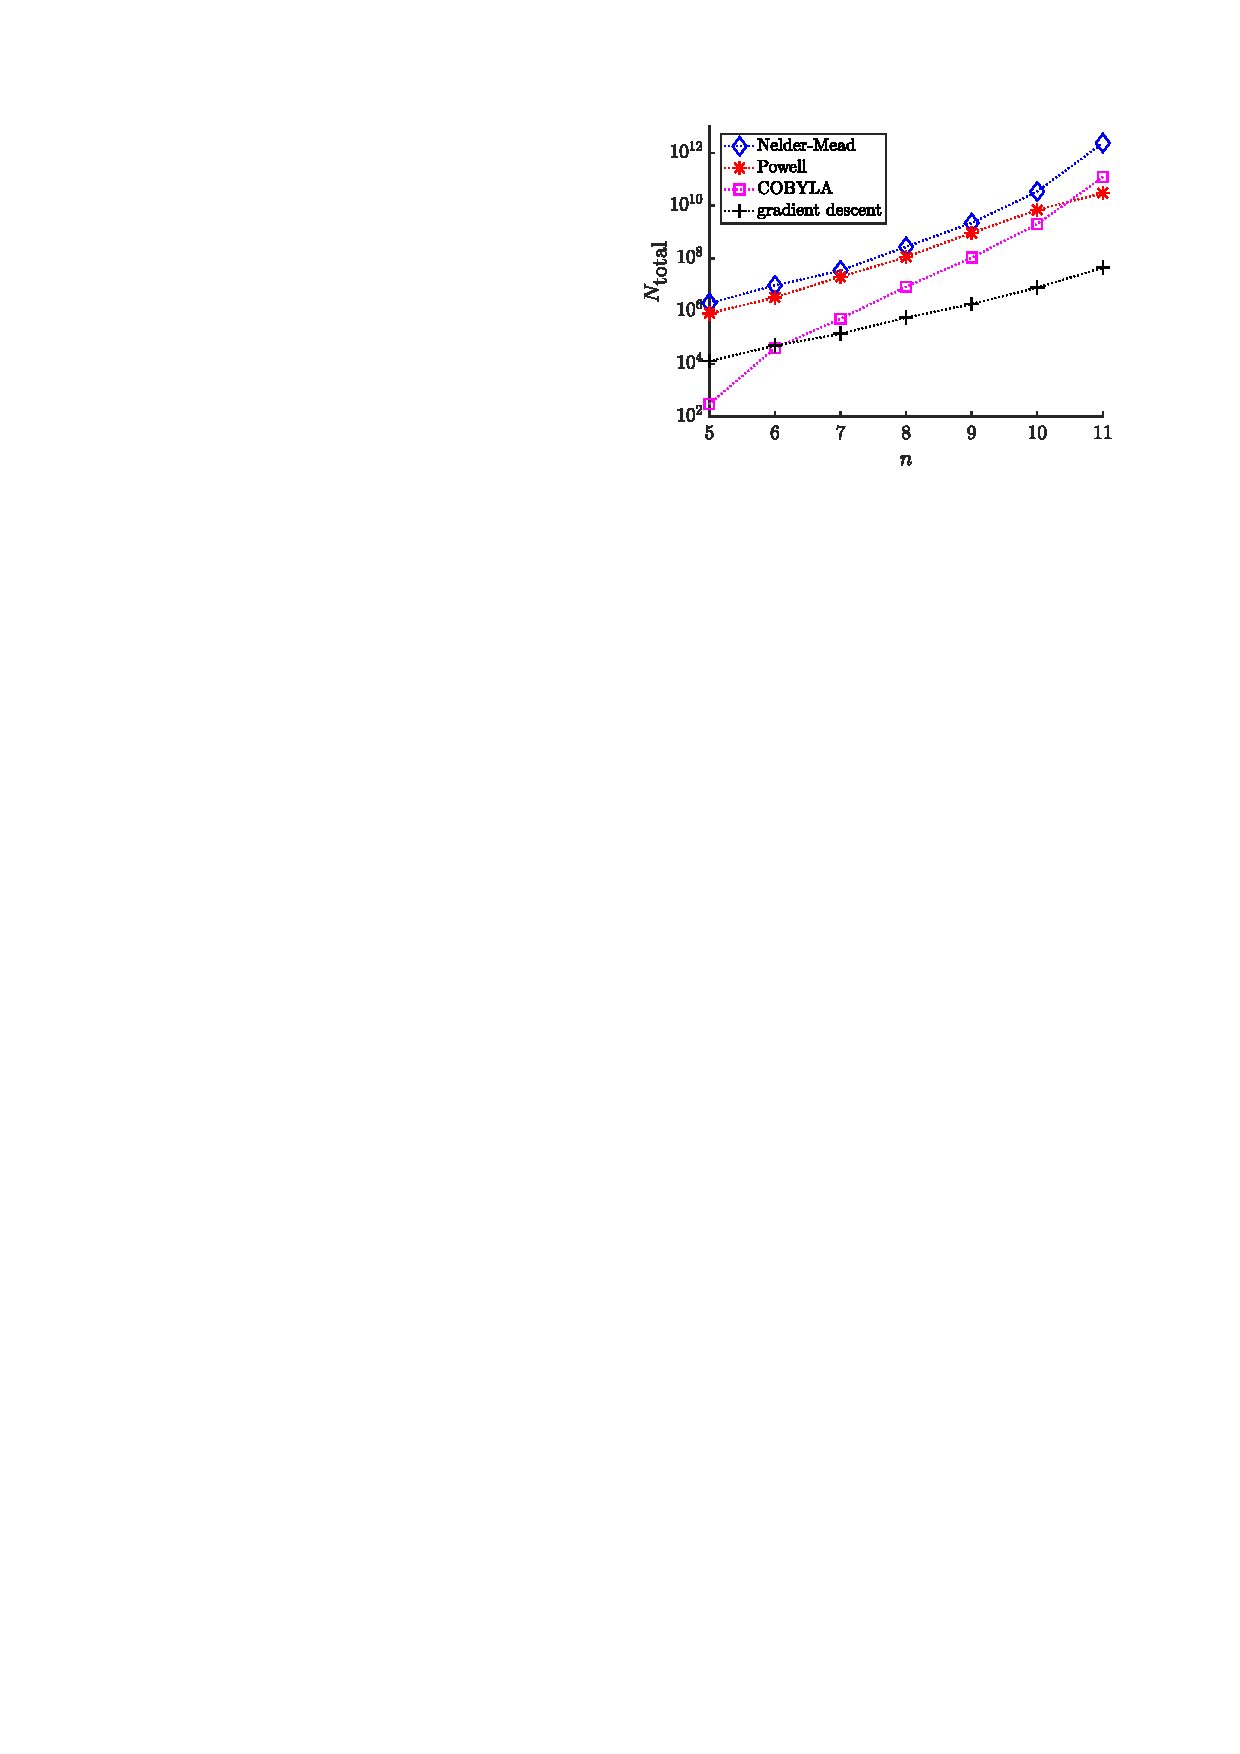
\includegraphics[width=12cm]{bp-nshots.pdf}
    \caption{バレンプラトーにおいて必要なオブザーバブルの測定回数 $N_{\text{total}}$の量子ビット数 $n$ に対する変化~\cite{arrasmith2021effect}。Nelder-Mead・Powell・COBYLA は勾配を用いないオプティマイザーである。}
    \label{fig:bp-var}
\end{figure}


% 実際にバレンプラトーが起きているときに必要な測定回数の変化を、図~\ref{fig:bp-var}に示す。
% \begin{figure}[H]
%     \label{fig:bp-var}
%     \centering
%     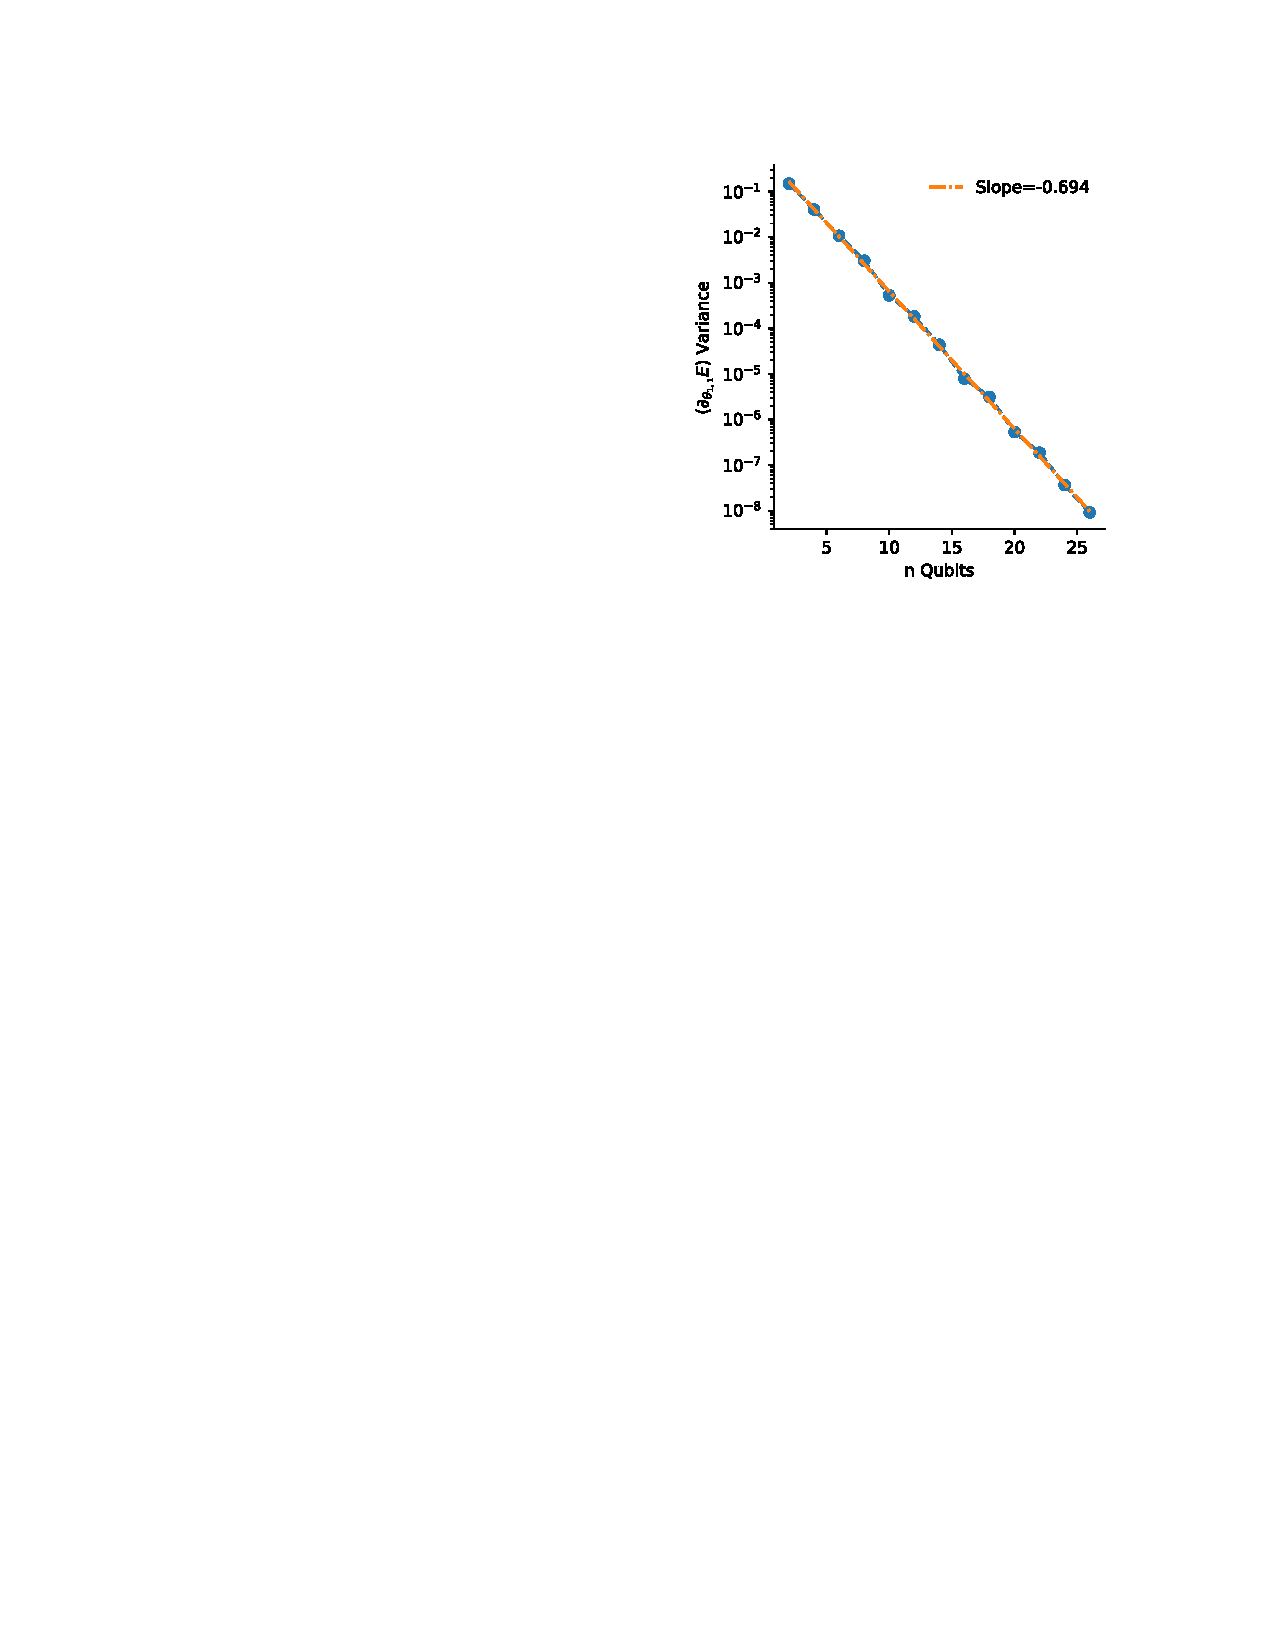
\includegraphics[width=8cm]{bp-var.pdf}
%     \caption{\cite{mcclean2018barren}}
% \end{figure}


\subsection{原因}\label{subsec:bp-cause}
バレンプラトーの原因として既に知られているものを以下に挙げる。
\begin{itemize}
    \item 学習回路の深さ・学習回路の表現能力・学習回路の生成するエンタングルメント~\cite{mcclean2018barren,cerezo2021cost,holmes2022connecting,marrero2021entanglement,leone2022practical}
    \item オブザーバブルの局所性~\cite{cerezo2021cost,uvarov2021barren}
    \item ノイズ~\cite{wang2021noiseinduced}
    \item データの入力~\cite{thanasilp2022exponential,thanasilp2021subtleties,leone2022practical}
\end{itemize}

バレンプラトーは、学習回路がユニタリ $2$--デザイン(\ref{sec:unitary-t-design}~節)という条件を満たすときに起きることが最初に示された~\cite{mcclean2018barren}。具体的な定理と証明については、付録の\ref{sec:bp-proof}~節に記す。
学習回路がユニタリ $2$--デザインを満たすことは、学習回路が深く、高い表現能力を持ち、多くのエンタングルメントを生成することを意味する。

オブザーバブルの局所性とは、測定するオブザーバブルが全量子ビットのうちいくつの量子ビットによって測定されるかを指す。グローバルオブザーバブルとは、全量子ビットの状態によって測定されるオブザーバブルのことであり、例えば、$Z\otn{n}$ である。ローカルオブザーバブルとは、全量子ビット数 $n$ に依存しない $m$ 個の量子ビットよって測定されるオブザーバブルのことである。例えば、$Z\otn{m}$ である。また、ローカルオブザーバブルの線形和もローカルオブザーバブルである。

ここで、量子回路の構造・量子ビット数 $n$・量子回路の層数 $L$・オブザーバブルの局所性がコスト関数の勾配の分散に与える影響を再現したものを示す。量子回路の構造として図~\ref{fig:tpa-hea-circuit}にあるように、Tensor Product Ansatz (TPA) と Hardware Efficient Ansatz (HEA) を用いた。

\begin{figure}[H]
    \centering
    \begin{tikzpicture}
        \node[scale=0.9]{
        \begin{quantikz}
            \lstick{$\ket{0}$}\slice{} & \gate{R_x(\th_{l,1})} & \gate{R_y(\th_{l,5})}\slice{$\times L$}& \meter{}\\
            \lstick{$\ket{0}$}         & \gate{R_x(\th_{l,2})} & \gate{R_y(\th_{l,6})}                & \meter{}\\
            \lstick{$\ket{0}$}         & \gate{R_x(\th_{l,3})} & \gate{R_y(\th_{l,7})}                & \meter{}\\
            \lstick{$\ket{0}$}         & \gate{R_x(\th_{l,4})} & \gate{R_y(\th_{l,8})}                & \meter{}
        \end{quantikz}
        \qquad\qquad
        \begin{quantikz}
            \lstick{$\ket{0}$}\slice{} & \gate{R_x(\th_{l,1})} & \gate{R_y(\th_{l,5})} & \ctrl{1}&  \qw    & \qw\slice{$\times L$}&\meter{}\\
            \lstick{$\ket{0}$}         & \gate{R_x(\th_{l,2})} & \gate{R_y(\th_{l,6})} & \targ{} & \ctrl{1}&\qw                &\meter{}\\
            \lstick{$\ket{0}$}         & \gate{R_x(\th_{l,3})} & \gate{R_y(\th_{l,7})} & \qw     & \targ{} &\ctrl{1}           &\meter{}\\
            \lstick{$\ket{0}$}         & \gate{R_x(\th_{l,4})} & \gate{R_y(\th_{l,8})} & \qw     &   \qw   &\targ{}            &\meter{}
        \end{quantikz}
        };
    \end{tikzpicture}
    \caption{TPA(左)と HEA(右)の量子回路}
    \label{fig:tpa-hea-circuit}
\end{figure}

\begin{figure}[H]
    \begin{minipage}[b]{0.5\columnwidth}
        \centering
        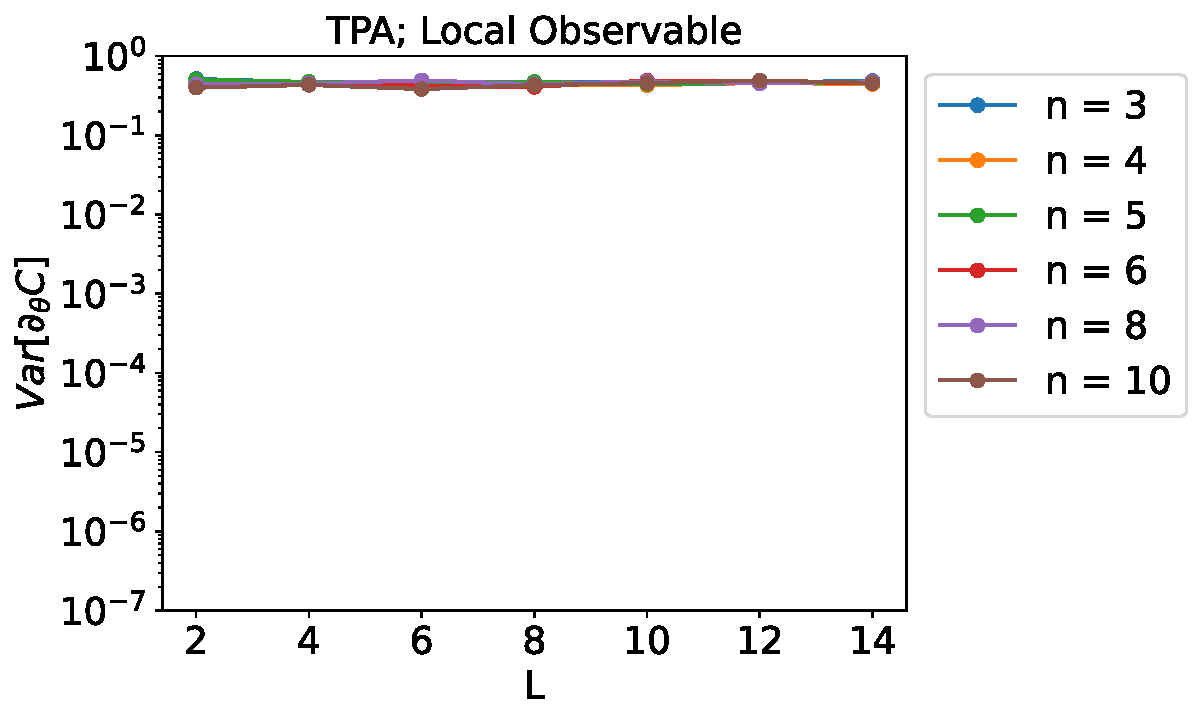
\includegraphics[width=8.5cm]{TPA-local-ob.pdf}
    \end{minipage}
    \hspace{0\columnwidth}
    \begin{minipage}[b]{0.5\columnwidth}
        \centering
        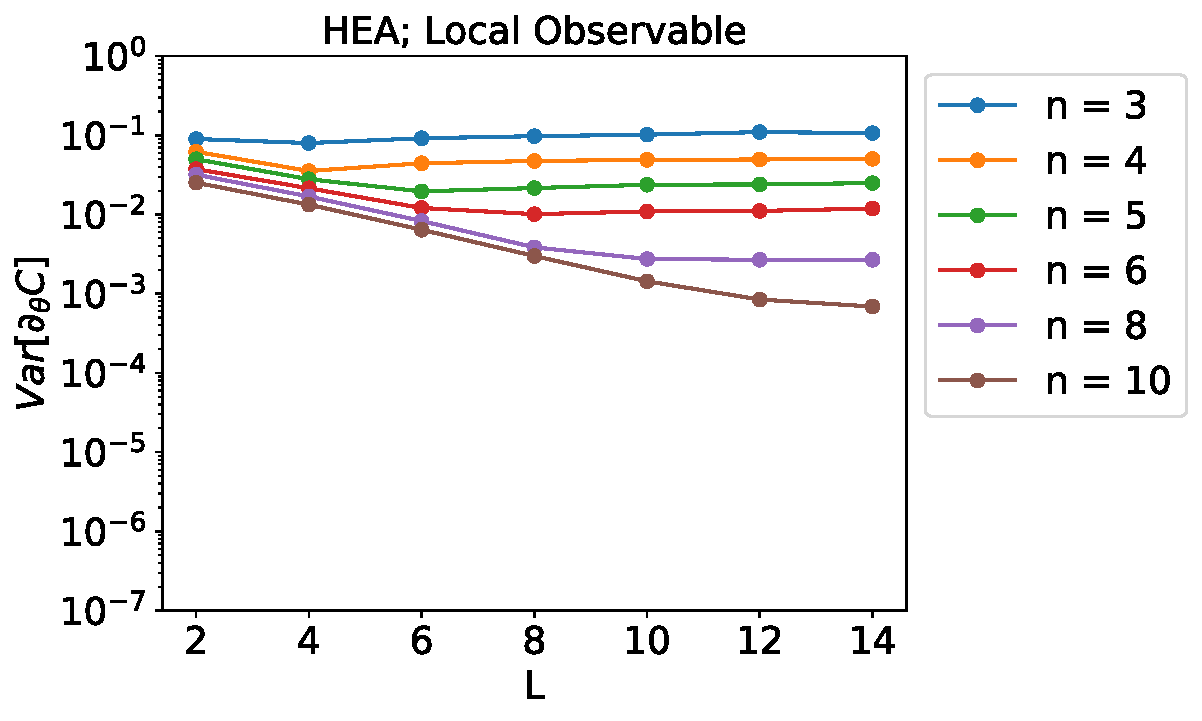
\includegraphics[width=8.5cm]{HEA-local-ob.pdf}
    \end{minipage}
\end{figure}
\begin{figure}[H]
    \begin{minipage}[b]{0.5\columnwidth}
        \centering
        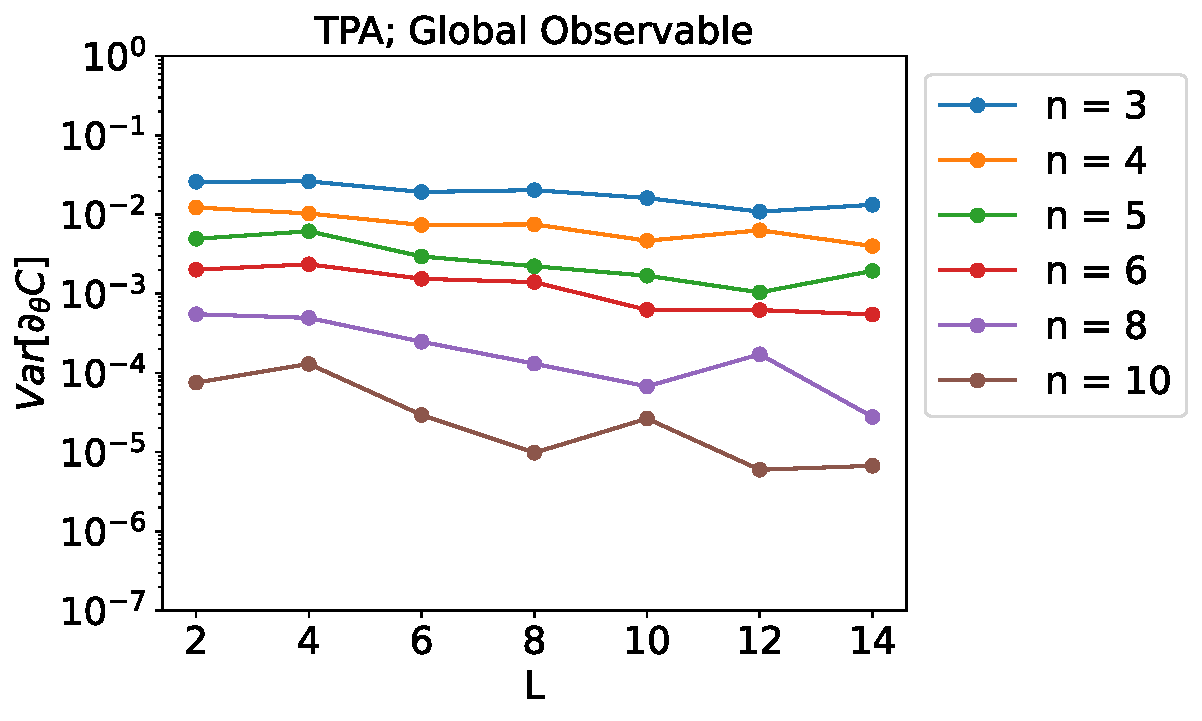
\includegraphics[width=8.5cm,height=5cm]{TPA-global-ob.pdf}
    \end{minipage}
    \hspace{0\columnwidth}
    \begin{minipage}[b]{0.5\columnwidth}
        \centering
        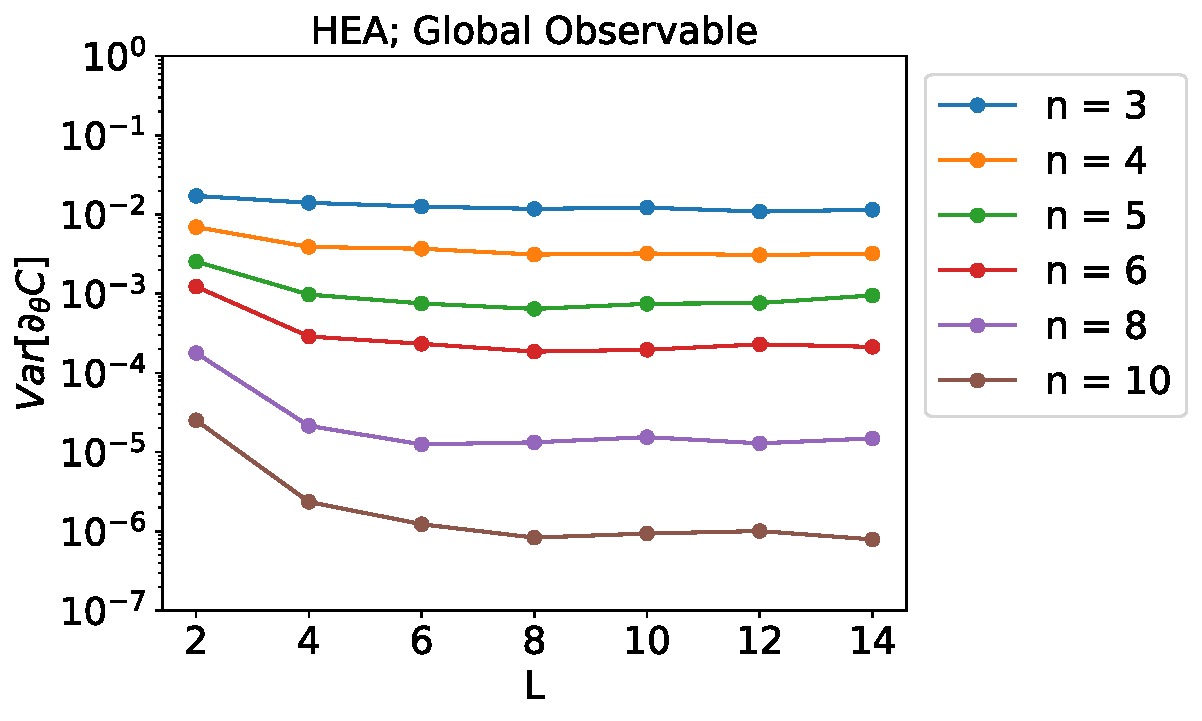
\includegraphics[width=8.5cm,height=5cm]{HEA-global-ob.pdf}
    \end{minipage}
    \caption{それぞれのプロットの横軸は量子回路の各層数 $L$、縦軸はコスト関数の勾配の分散を表す。上段は、TPA(左)と HEA(右)に対してローカルオブザーバブル $Z\ot I \ot\cdots\ot I$ を用いた場合の勾配の分散の変化を示している。下段は、グローバルオブザーバブル $\dyad{0}\otn{n}$ を用いた場合のそれぞれの量子回路における勾配の分散の変化を示している。}
    \label{fig:var-ob}
\end{figure}

図~\ref{fig:var-ob}において、上段は、Tensor Product Ansatz (TPA)(左)と Hardware Efficient Ansatz (HEA)(右)に対してローカルオブザーバブル $Z\ot I \ot\cdots\ot I$ を用いた場合の、各量子ビット数 $n$ と量子回路の各層数 $L$ に対する勾配の分散の変化を示している。下段は、グローバルオブザーバブル $\dyad{0}\otn{n}$ を用いた場合の勾配の分散の変化を示している。これらの図から、エンタングルメントを多く生成すること、層数 $L$ を増やすこと、グローバルオブザーバブルを用いることはいずれも、勾配の分散のスケールをより小さくすることがわかる。


\subsection{回避方法}
豊かな表現能力を持ち、エンタングルメントを多く生成するような深い量子回路を用いることと、グローバルオブザーバブルを用いることは、パラメーターの探索すべき領域を指数関数的に増大させるため、バレンプラトーを引き起こすと考えられている。よって、バレンプラトーを回避するためには、学習回路の深さ・表現能力・エンタングルメントを抑えて、ローカルオブザーバブルを用い、かつ、学習回路の表現領域にコスト関数の最適解があるようにその構造を設計する必要がある。
これらの原因を考慮して、バレンプラトーを回避するための方法がいつくか提案されている。
\begin{itemize}
    \item ローカルオブザーバブルを用いる~\cite{cerezo2021cost}。これにより、データ入力がない場合は、学習回路の深さが $\order{\log{n}}$ であればバレンプラトーは起きないことが示されている。
    \item 学習回路の各層ごとにパラメーターを最適化する~\cite{skolik2021layerwise}。これにより、実質的な学習回路の深さを減らすことができる。
    \item 一部の学習パラメーターの初期値を残りの回路と打ち消し合うように設定する~\cite{grant2019initialization}。これにより、実質的な学習回路の深さを減らすことができる。
    \item 学習パラメーター間に相関を持たせる~\cite{holmes2022connecting}。これにより、学習回路の表現能力を抑えることができる。
    \item 学習パラメーターの初期値を、一様分布ではなく、正規分布からサンプリングする~\cite{zhang2022escaping}。
\end{itemize}

また、QAOA では、最適なパラメーターがあるパターンを持つことが先行研究\cite{zhou2020quantum}で示された。このパターンに近いパラメーターを初期値として用いることで、ランダムにパラメーターを選んだ場合よりも学習が早くなることも示されている。
また、Quantum Tree Tensor Network (QTTN) や Quantum Convolutional Neural Network (QCNN) はその構造上、バレンプラトーが起きないことが示されている\cite{cong2019quantum,martin2022barren}。

しかしながら、バレンプラトーを避けることだけできれば良いわけではない。というのも、例えば、バレンプラトーを避けるためにエンタングルメントが生じない量子回路を用いたとすると、その量子回路は古典コンピューターによって効率的にシミュレーションすることができる。よって、変分量子アルゴリズムにおいて古典計算よりも効率的な計算を行うためには、バレンプラトーを避ける一方で、古典コンピューターによるシミュレーションが困難な量子回路を用いる必要がある。
